\documentclass[12pt]{article}
\usepackage[utf8]{inputenc}
\usepackage[margin=0.65in]{geometry}
\usepackage{minted}
\usepackage{upquote}
\usepackage{parskip}
\usepackage{xcolor}
\definecolor{LightGray}{gray}{0.97}
\renewcommand{\baselinestretch}{1.21}
\setminted[python]{baselinestretch=1.2,tabsize=4,bgcolor=LightGray,fontsize=\footnotesize,linenos}
\setminted[bash]{baselinestretch=1.2,bgcolor=LightGray,fontsize=\footnotesize,linenos}
\usepackage{amsmath}
\usepackage{graphicx}
\definecolor{bg}{rgb}{0.95,0.95,0.95}

\usepackage{hyperref}

\graphicspath{{/}}

%Documents what you did for your project and how.
%Describe the problem, how you try to solve the problem, and your results. 

\begin{document}

\begin{center}
\section*{Final Project Report}
Joon Hee Lee - s171507
\end{center}

\section*{Chosen Project}

Worksheet 10: Environment Mapping and Bump Mapping

The goal of this project is to use a cube map to render an environment and a curved reflector. We also use bump mapping to add surface details to the reflector.

\section*{Part 1: Cube Map}

The goal of this part is to use a cube map to texture a sphere.

We begin with the textured sphere (2D texture) from the end result of Worksheet 6 Part 3, which looks like:

\begin{center}
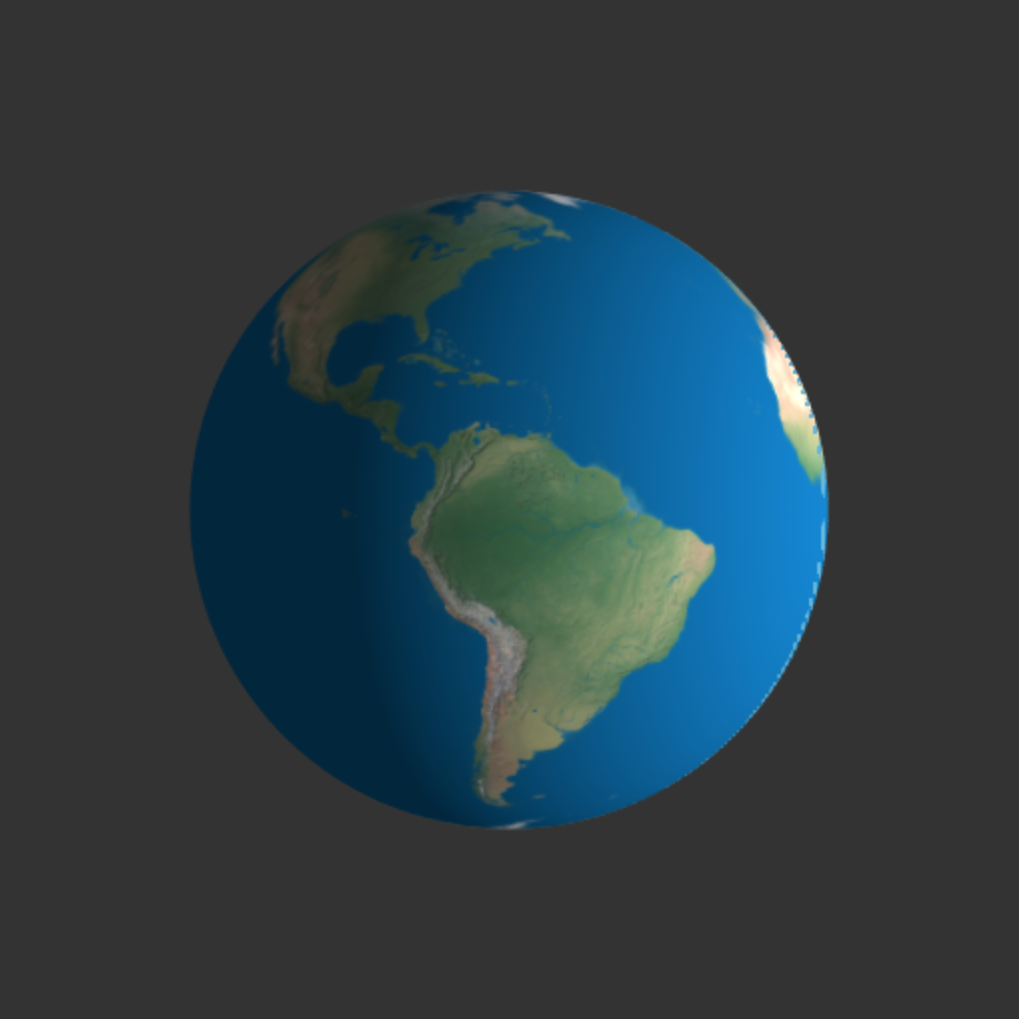
\includegraphics[scale=0.35]{images/earth}
\end{center}

Now, we must replace the 2D texture with a cube map texture using the images in the provided \texttt{textures.zip}. Thus, we create an array \texttt{cubemap} of the 6 images that will texture the sphere, and a corresponding array \texttt{cubemapSides} which label which face of the cube each image belongs to:


\begin{minted}[linenos=true,bgcolor=bg]{js}
var cubemap = ['textures/cm_left.png', // POSITIVE_X
               'textures/cm_right.png', // NEGATIVE_X
               'textures/cm_top.png', // POSITIVE_Y
               'textures/cm_bottom.png', // NEGATIVE_Y
               'textures/cm_back.png', // POSITIVE_Z
               'textures/cm_front.png']; // NEGATIVE_Z 
               
var cubemapSides = [gl.TEXTURE_CUBE_MAP_POSITIVE_X,
                    gl.TEXTURE_CUBE_MAP_NEGATIVE_X,
                    gl.TEXTURE_CUBE_MAP_POSITIVE_Y,
                    gl.TEXTURE_CUBE_MAP_NEGATIVE_Y,
                    gl.TEXTURE_CUBE_MAP_POSITIVE_Z,
                    gl.TEXTURE_CUBE_MAP_NEGATIVE_Z];
\end{minted}

Then, we initialize a texture object for the cubemap, and assign it to \texttt{TEXTURE0}:

\begin{minted}[linenos=true,bgcolor=bg]{js}
var cubeMap = gl.createTexture();
gl.activeTexture(gl.TEXTURE0);
gl.bindTexture(gl.TEXTURE_CUBE_MAP, cubeMap);
gl.uniform1i(gl.getUniformLocation(program, "texMap"), 0);
gl.texParameteri(gl.TEXTURE_CUBE_MAP, gl.TEXTURE_MIN_FILTER,gl.NEAREST);
gl.pixelStorei(gl.UNPACK_FLIP_Y_WEBGL, true);
\end{minted}

Now, we must load in all 6 images in a \texttt{for} loop. To do this, we create a variable \texttt{cubeMapSidesLoaded} which will count how many images have been loaded. When all images have been loaded, we will call \texttt{render()}. After we load each image, we assign it to the appropriate face of the cube map:

\begin{minted}[linenos=true,bgcolor=bg]{js}
for (var i = 0; i < cubemap.length; i++) {
    var image = document.createElement('img');
    image.cubemapSide = cubemapSides[i];
    image.crossorigin = 'anonymous';
    image.onload = function(event) {
        var image = event.target;
        cubeMapSidesLoaded += 1;
        gl.texImage2D(image.cubemapSide, 0, gl.RGBA, gl.RGBA,
                      gl.UNSIGNED_BYTE, image);
        if (cubeMapSidesLoaded == cubemap.length) {
            render();
        }
    }
    image.src = cubemap[i];
}
\end{minted}

One last thing to change is to change the type of \texttt{texMap} from \texttt{sampler2D} to \texttt{samplerCube} in the fragment shader. The projection and view matrices we will use are as follows:

\begin{minted}[linenos=true,bgcolor=bg]{js}
var projectionMatrix = perspective(
    90.0, canvas.width/canvas.height, 0.0001, 100)

var eye = vec3(0, 0, cameraRadius);
var at = vec3(0, 0, 0);
var up = vec3(0.0, 1.0, 0.0);
var viewMatrix = lookAt(eye, at, up);
\end{minted}

The result is the following:

\begin{center}
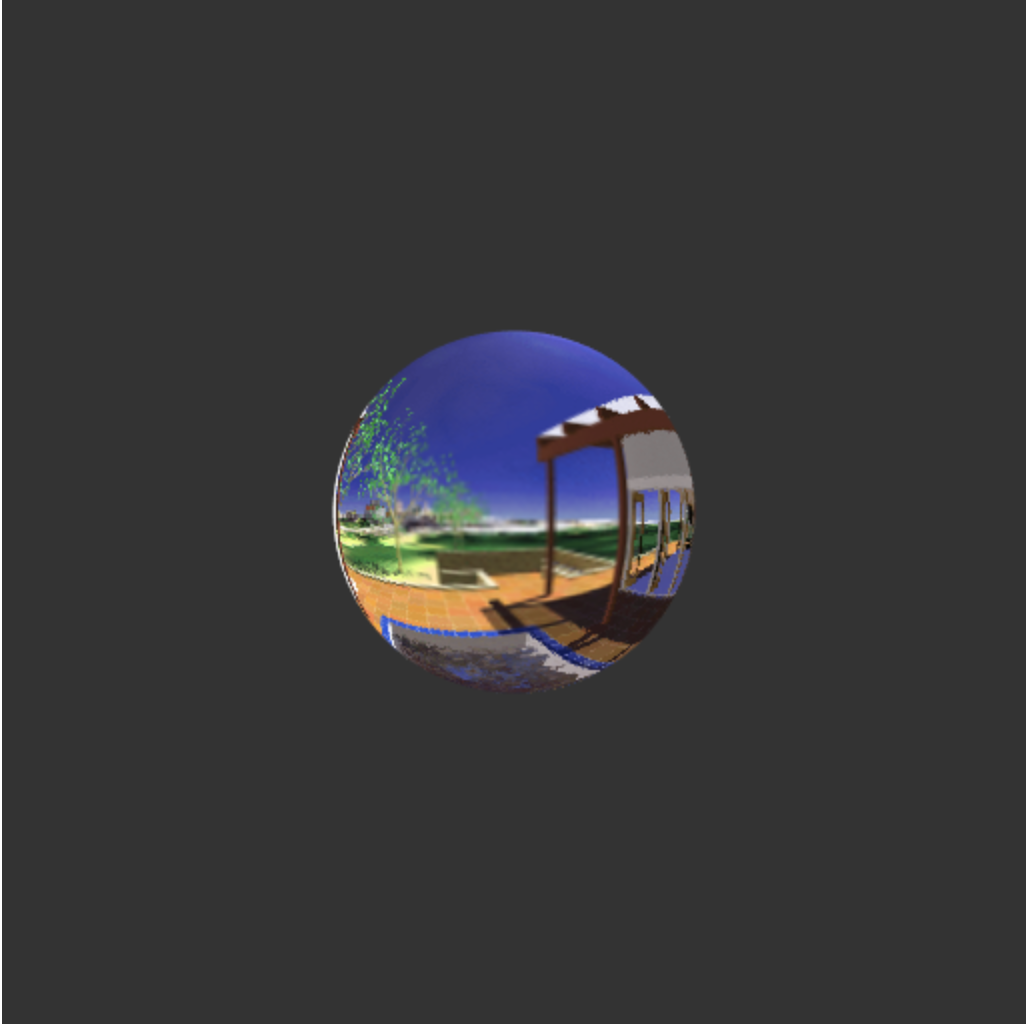
\includegraphics[scale=0.5]{images/part1}
\end{center}

\newpage

\section*{Part 2: Environment}

The goal of this part is to draw the environment in the background using the cube map.

First, we must draw a screen-filling quad at the far plane of the view frustum. The coordinates of the quad, in clip space coordinates, are:

\begin{minted}[linenos=true,bgcolor=bg]{js}
const background_points = [
    vec4(-1.0, -1.0, 0.999, 1.0),
    vec4(1.0, -1.0, 0.999, 1.0),
    vec4(-1.0, 1.0, 0.999, 1.0),
    vec4(1.0, 1.0, 0.999, 1.0),
]
\end{minted}

When we buffer vertices, we buffer the sphere's points (\texttt{pointsArray}) along with the background points as follows:

\begin{minted}[linenos=true,bgcolor=bg]{js}
gl.bufferData(gl.ARRAY_BUFFER,
    flatten(pointsArray.concat(background_points)), gl.STATIC_DRAW);
\end{minted}

Now, we introduce a uniform matrix $M_{tex}$ that transforms vertex positions to texture coordinates. For the sphere vertices, $M_{tex}$ is simply a uniform matrix. However, since the background quad's vertices are in clip space coordinates, its model-view-projection matrix is an identity matrix, while $M_{tex}$ should transform from clip space positions to world space directions. 

Since $CLIP = PROJ \times VIEW \times WORLDSPACE$, and we want $M_{tex} \times CLIP = WORLDSPACE$, we have $M_{tex} = VIEW^{-1} \times PROJ^{-1}$. However, for the view matrix, we only consider the rotational part since the background is far away and we can disregard the translational part. The rotational part of the view matrix is simply the top left $3 \times 3$ corner. Thus, we can compute $M_{tex}$ for the background points as follows:

\begin{minted}[linenos=true,bgcolor=bg]{js}
var viewMatrixRot = mat4(
    vec4(viewMatrix[0][0], viewMatrix[0][1], viewMatrix[0][2], 0),
    vec4(viewMatrix[1][0], viewMatrix[1][1], viewMatrix[1][2], 0),
    vec4(viewMatrix[2][0], viewMatrix[2][1], viewMatrix[2][2], 0),
    vec4(0.0, 0.0, 0.0, 1.0)
);

var mtex = mult(inverse(viewMatrixRot), inverse(projectionMatrix));
\end{minted}
\newpage
Then we can draw the background points:

\begin{minted}[linenos=true,bgcolor=bg]{js}
gl.disable(gl.DEPTH_TEST);
gl.uniformMatrix4fv(
    gl.getUniformLocation(program, "mTex"), false, flatten(mtex));
gl.uniformMatrix4fv(projectionMatrixLocation, false, flatten(mat4()));
gl.uniformMatrix4fv(viewMatrixLocation, false, flatten(mat4()));
gl.uniformMatrix4fv(modelMatrixLocation, false, flatten(mat4()));
gl.drawArrays(
    gl.TRIANGLE_STRIP, pointsArray.length, background_points.length);
gl.enable(gl.DEPTH_TEST);
\end{minted}

Note that we disable depth testing when drawing the background points, since setting $w = 1$ for the points was causing problems with rendering.

When we draw the sphere, we set $M_{tex}$ to an identity matrix and set the other matrices to their default values:

\begin{minted}[linenos=true,bgcolor=bg]{js}
gl.uniformMatrix4fv(
    gl.getUniformLocation(program, "mTex"), false, flatten(mat4()));        
gl.uniformMatrix4fv(
    projectionMatrixLocation, false, flatten(projectionMatrix));
gl.uniformMatrix4fv(viewMatrixLocation, false, flatten(viewMatrix));
gl.uniformMatrix4fv(
    modelMatrixLocation, false, flatten(translate(0, 0, 0)));
gl.drawArrays( gl.TRIANGLES, 0, pointsArray.length);
\end{minted}

The following line is added in the fragment shader to enable the use of the uniform variable \texttt{mTex}:

\begin{minted}[linenos=true,bgcolor=bg]{glsl}
uniform mat4 mTex;
\end{minted}

The result we get is as follows:

\begin{center}
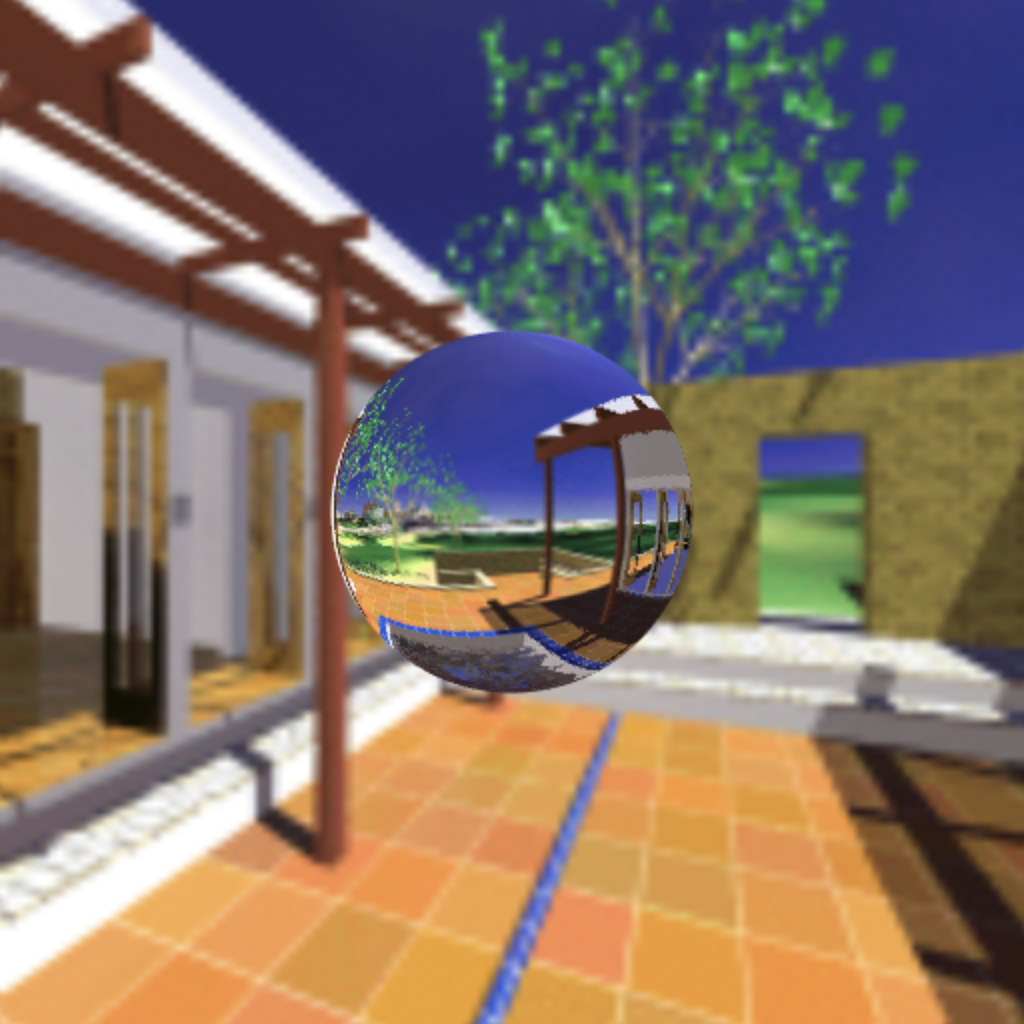
\includegraphics[scale=0.4]{images/part2}
\end{center}

\newpage

\section*{Part 3: Reflection}

The goal of this part is to turn the sphere into a reflector. Currently it is looking up the environment in the normal direction rather than the direction of reflection.

In the fragment shader, we create two new uniform variables:

\begin{minted}[linenos=true,bgcolor=bg]{glsl}
uniform bool reflexive;
uniform vec3 eye;
\end{minted}

The boolean \texttt{reflexive} is \texttt{true} for the sphere and \texttt{false} for the environment. We update the new uniform variables in the javascript \texttt{render()} function as follows:

\begin{minted}[linenos=true,bgcolor=bg]{js}
// While Rendering Environment
gl.uniform1f(gl.getUniformLocation(program, "reflexive"), 0);

// While Rendering Sphere
gl.uniform1f(gl.getUniformLocation(program, "reflexive"), 1);
gl.uniform3fv(gl.getUniformLocation(program, "eye"), flatten(eye));   
\end{minted}

We can compute the direction of reflection using the GLSL function \texttt{reflect(vec3 incident, vec3 normal)}. The direction of incidence in is simply $-eye$.

Thus, the fragment coloring logic is as follows:

\begin{minted}[linenos=true,bgcolor=bg]{glsl}
vec3 texCoord = (mTex * vNormal).xyz;
if (reflexive) {
    gl_FragColor = textureCube(texMap, reflect(-eye, texCoord));
}
else {
    gl_FragColor = textureCube(texMap, texCoord);
}
\end{minted}

The result of this looks like this:

\begin{center}
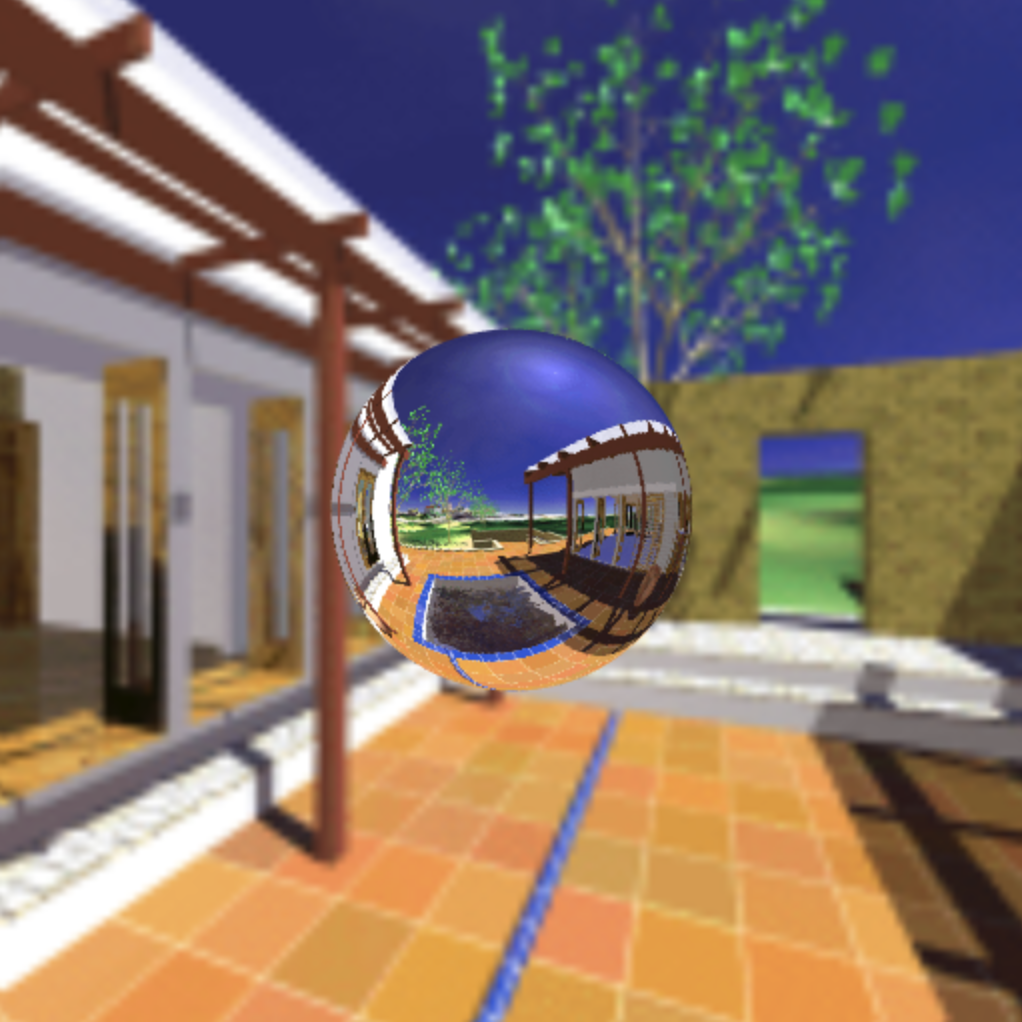
\includegraphics[scale=0.39]{images/part3}
\end{center}

\newpage

\section*{Part 4: Bump Mapping}

The goal of this part is to perturb the normal of the mirror ball using a normal map to give the impression that the ball surface is bumpy.

First, we load the normal map image from \texttt{normalmap.png} and bind it to \texttt{TEXTURE1}. The details of this is identical to Worksheet 6 Part 3 so it will not be explained fully. We create a uniform variable \texttt{texMap2} so that we can access the normal map from the fragment shader.

As in Worksheet 6 Part 3, we can calculate the $uv$ coordinates of each fragment as follows:

\begin{minted}[linenos=true,bgcolor=bg]{glsl}
float u = atan(vNormal.x, vNormal.z) / (-2.0 * PI);
float v = atan(
    sqrt(vNormal.z * vNormal.z + vNormal.x * vNormal.x), vNormal.y) / PI;
\end{minted}

Since the color in the normal map is in the range [0, 1], we must transform it to the range [-1, 1] to get the actual normal, which is in tangent space. Thus, we have:

\begin{minted}[linenos=true,bgcolor=bg]{glsl}
vec3 tangent_vector = (2.0 * texture2D(texMap2, vec2(u, v)) - 1.0).xyz;
\end{minted}

Since this normal is in tangent space, we transform it to world space as follows:

\begin{minted}[linenos=true,bgcolor=bg]{glsl}
vec3 newNormal = rotate_to_normal(vNormal.xyz, tangent_vector);
\end{minted}

We then use this new normal in place of the sphere's real normals in the rest of the process (remember that \texttt{mTex} is simply a identity matrix):

\begin{minted}[linenos=true,bgcolor=bg]{glsl}
vec3 texCoord = (mTex * vec4(newNormal, 1.0)).xyz;    
gl_FragColor = textureCube(texMap, reflect(-eye, texCoord));
\end{minted}

The end result is as follows:

\begin{center}
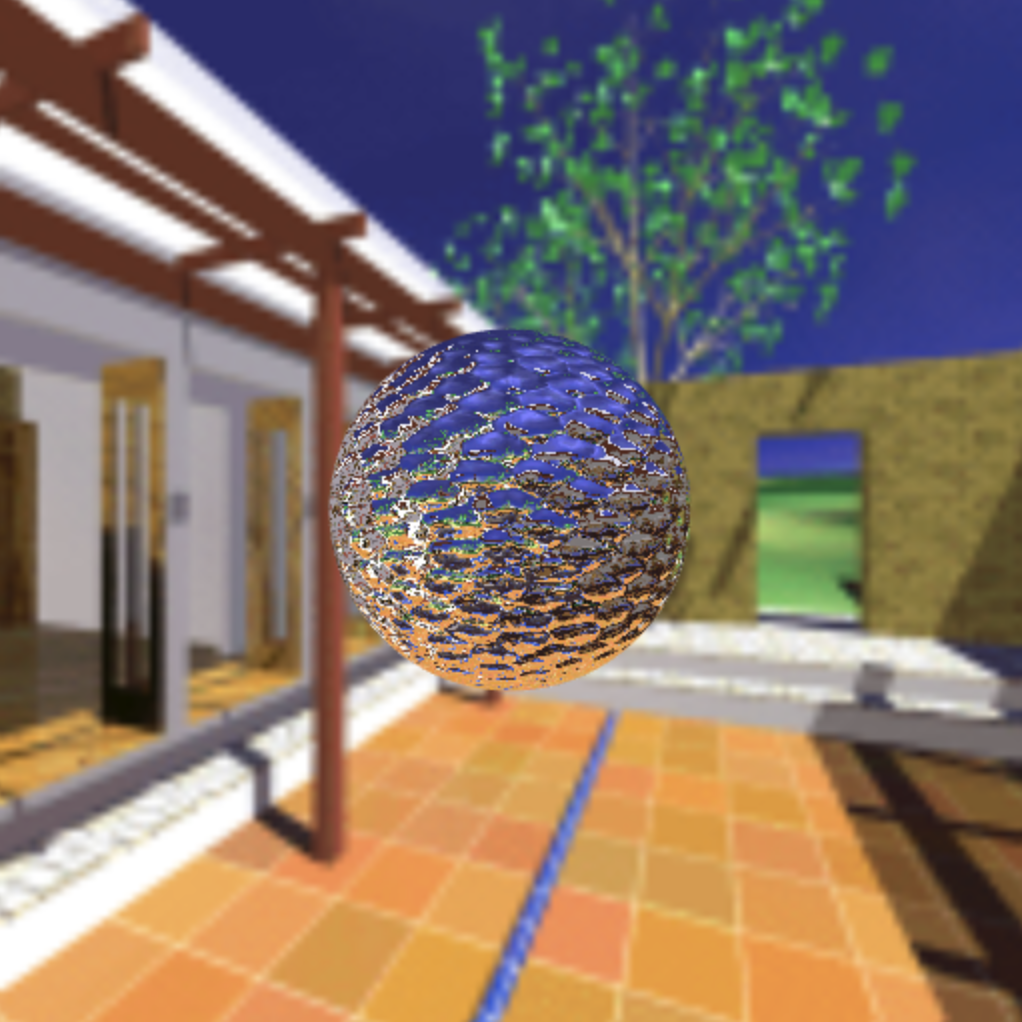
\includegraphics[scale=0.4]{images/part4}
\end{center}



\end{document}
